\section{模型讨论}
\subsection{数据拟合结果及分析}
\subsubsection{数据源}
\par 拟合所用数据为2020年1月20日至5月1日官方发布的全国疫情数据。
以下为官方发布的疫情数据:
\begin{figure}[H]
    \centering
    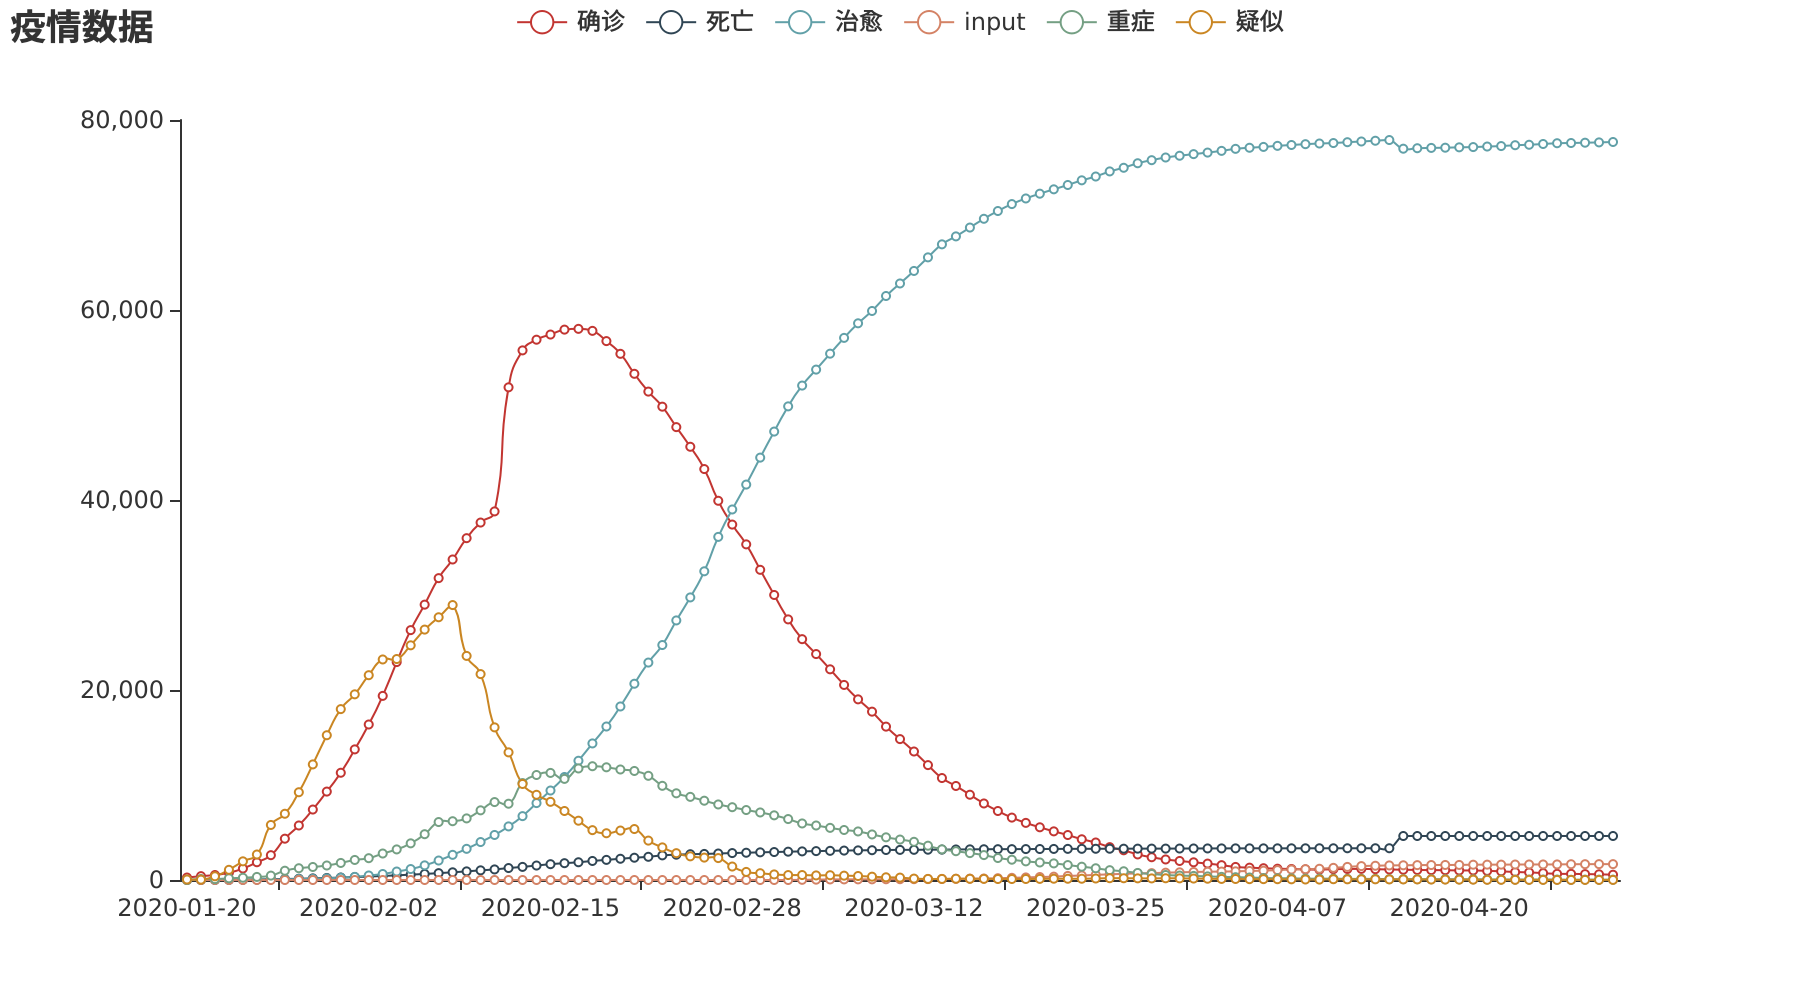
\includegraphics[width=\imagewidth]{疫情数据.png}
    \caption{全国疫情数据}
\end{figure}
\begin{figure}[H]
    \centering
    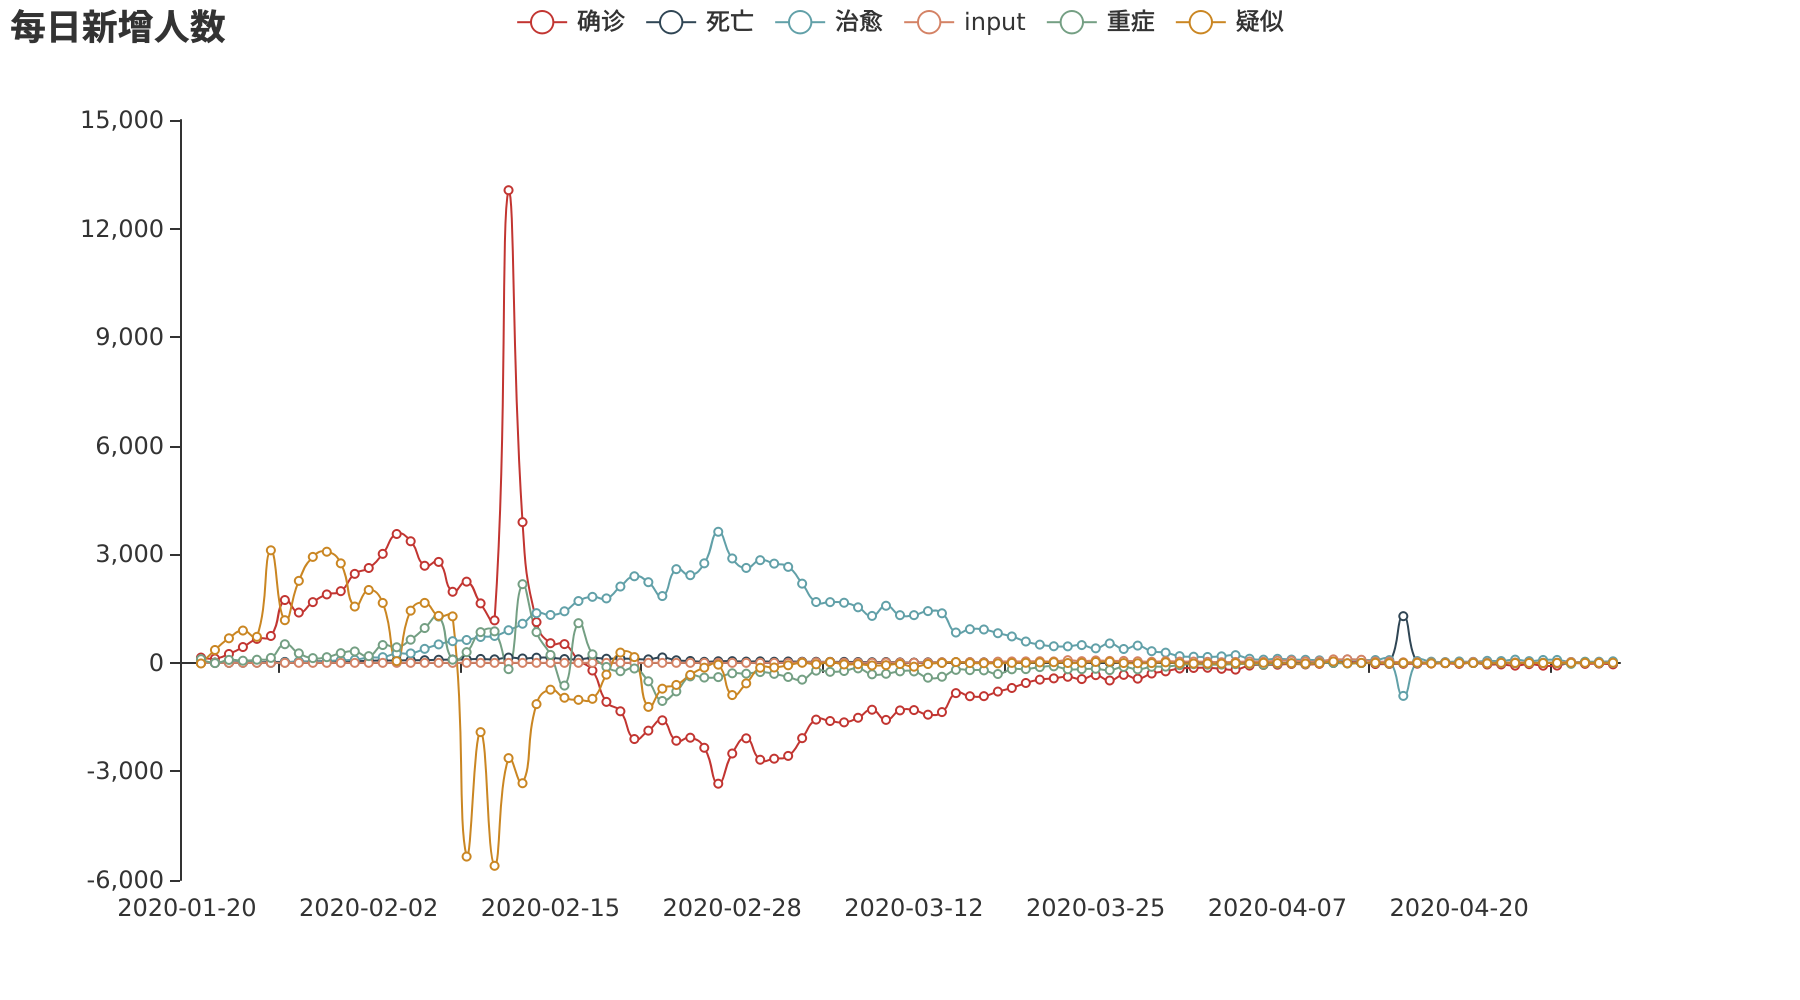
\includegraphics[width=\imagewidth]{每日新增人数.png}
    \caption{每日新增人数}
\end{figure}
\par
2月12日确诊人数猛增,
是因为当日重新规定了确诊条件,
导致许多疑似病例纳入确诊人数。
\subsubsection{拟合方法}
\par 本文采取$L-BFGS-B$方法对每个模型进行拟合,
将每个模型的预测值与真实数据进行对比,
并给出拟合后的参数以及损失值$LOSS$,
损失值将作为评判模型拟合优劣的指标之一。
\par 损失值定义:
\begin{equation}
    LOSS = \frac{\sum\limits^{day}\sum\limits^{group}
        \left|True-Predict\right|}{day}
\end{equation}
\subsubsection{SIR模型拟合结果}
\showtable{SIR}
\showfigure{SIR}
\par $SIR$模型中$\P{S}{I}$为感染人数增长率,
不同于感染率。
$\P{I}{R}$为治愈人数增长率,
不同于治愈率。
\subsubsection{SEIR模型拟合结果}
\showtable{SEIR}
\showfigure{SEIR}
\par $SEIR$模型中$\P{E}{R}$极低,
一可理解为潜伏期较长,
二可理解为致病率较高,
这两点都与实际情况吻合。
\subsubsection{SEIRD模型拟合结果}
\showtable{SEIRD}
\showfigure{SEIRD}
\par $SEIRD$模型中$\P{I}{D}$为死亡人数增长率,
不同于死亡率。
\subsubsection{SEIRS模型拟合结果}
\showtable{SEIRS}
\showfigure{SEIRS}
\par $SEIRS$模型中的$\P{R}{I}=0.001$,
可以理解为复阳率极低,
说明复阳人数占患病人数比例极低,
对疫情的影响微乎其微。
\par 对比各个模型拟合前后的参数值变化:
\showtables{SIR}
\showfigures{SIR}
$\P{S}{I}$有所下降,
$\P{I}{R}$有所增减,
代表感染率降低,
治愈率提高。
\showtables{SEIR}
\showfigures{SEIR}
$\P{S}{E},\P{E}{I}$有所下降,
$\P{I}{R}$有所增减,
代表感染率降低,
治愈率提高。
\showtables{SEIRD}
\showfigures{SEIRD}
$\P{S}{E}$稍有增加,
$\P{E}{I}$有所下降,
$\P{S}{E}\cdot \P{E}{I}$有所下降,
$\P{I}{R}$有所增减,
$\P{I}{D}$有所下降
代表患病率降低,
治愈率提高,
死亡率降低。
\showtables{SEIRS}
\showfigures{SEIRS}
$SEIRS$模型与$SEIRD$模型的参数十分接近,
无论分段与否,$SEIRS$模型的$\P{S}{I}$均为$0.001$,
说明$\P{S}{I}$对模型的影响极其微弱。
\subsection{结果分析}
\par 仅从$LOSS$值判断,
模型从优到劣排序为$SEIRD>SEIRS>SEIR>SIR$。
\par 参考$LOSS$值的大小,
认为在上述几种模型中,
$SEIRD$模型最适用于该类传染病预测。
\par 无论哪种模型,
比较模型分段前后参数,
均可得出传染病的传染率降低、治愈率增加、死亡率降低这一结论,
可以说明隔离措施十分有效。
\par 根据$SEIRD$模型的拟合参数,
可以计算出病毒大致的基础再生数
$R_0$\cite{应用SEIR模型预测2009年甲型H1N1流感流行趋势,王宝童2013流感传播数学模型的基本再生数}:
\begin{equation}
    R_0 = \frac{\P{S}{I}}{\P{I}{R}}
    = \frac{\P{S}{E}\cdot \P{E}{I}}{\P{I}{R}}
\end{equation}
\par 计算出隔离前$R_0=5.937$,隔离后$R_0=1.242$,可见疫情传播得到了有效的抑制。